\documentclass[conference]{IEEEtran}
\IEEEoverridecommandlockouts
% The preceding line is only needed to identify funding in the first footnote. If that is unneeded, please comment it out.
%Template version as of 6/27/2024

\usepackage{cite}
\usepackage{amsmath,amssymb,amsfonts}
\usepackage{algorithmic}
\usepackage[dvipdfmx]{graphicx}
\usepackage{textcomp}
\usepackage[dvipdfmx]{xcolor}

\usepackage{booktabs} 
\usepackage{caption} 
\usepackage{multirow}
\usepackage{makecell}

\def\BibTeX{{\rm B\kern-.05em{\sc i\kern-.025em b}\kern-.08em
    T\kern-.1667em\lower.7ex\hbox{E}\kern-.125emX}}

\begin{document}

\title{Multi-Channel based Light Inception with boosTing tEchniques for Time Series Classification}

\author{\IEEEauthorblockN{Sota Kobayashi}
\IEEEauthorblockA{\textit{Graduate School of Information Sciences} \\
\textit{Hiroshima City University}\\
Hiroshima, Japan\\
mm67012@e.hiroshima-cu.ac.jp}
\and
\IEEEauthorblockN{Keiichi Tamura}
\IEEEauthorblockA{\textit{Graduate School of Information Sciences} \\
\textit{Hiroshima City University}\\
Hiroshima, Japan\\
ktamura@hiroshima-cu.ac.jp}
}

\maketitle

\begin{abstract}
%近年，深層学習を用いた時系列データの分類に関する研究が盛んに行われている．時系列データの分類は，異常検知，予測，識別において重要な基礎技術であり，ヘルスケア，人間活動認識，サイバーセキュリティ，金融といった幅広い分野での応用が期待されている．時系列データを高精度に分類可能な深層モデルはいくつか存在するが，IoT機器などのエッジデバイスへの実装や，膨大なデータのリアルタイム処理，消費電力の削減という観点からは，モデルの精度を維持しつつ軽量化を図ることは必要不可欠である．
%本論文では，深さ単位分離可能畳み込み（Depthwise Separable Convolution）を用いた軽量モデルであるLight Inception with boosTing tEchniques (LITE)モデルに，MACDヒストグラムを組み合わせたMulti-Channel MACD-Histogram-based LITE (MC-MHLITE)モデル，およびそのアンサンブル型であるParallel-Multi-Channel MACD-Histogram-based LITE (PMC-MHLITE)モデルを提案する．これらにより，LITEモデルの軽量性を維持しつつ，異なる特徴量を活用することで分類精度の向上を図る．
Time series classification (TSC) is a fundamental technology for anomaly detection, prediction, and identification, and its application covers a wide range of fields including healthcare, human activity recognition, cybersecurity, and finance. Although there are a number of deep learning–based models that can accurately classify time series data, it is important to reduce the size of the model while maintaining accuracy for its implementation on edge devices, such as Internet of Things (IoT) devices. This allows for the real-time processing and reduces power consumption. In this paper, we propose two lightweight models: the Multi-Channel MACD-Histogram-based LITE (MC-MHLITE) model and its ensemble variant, the Parallel Multi-Channel MACD-Histogram-based LITE (PMC-MHLITE) model. In the MC-MHLITE model, MACD histogram is integrated into the Light Inception with boosTing tEchniques (LITE) model to enhance feature extraction. The PMC-MHLITE model is designed as a parallel architecture comprising multiple MC-MHLITE units to further improve the versatility of the classification performance. These models aim to improve accuracy by incorporating diverse features while maintaining the efficiency of the LITE model.
\end{abstract}

\begin{IEEEkeywords}
Time series classification, Deep learning, the Light Inception with boosTing tEchniques model, MACD histogram
\end{IEEEkeywords}

\section{Introduction}
%現在，ヘルスケア，人間活動認識（Human Activity Recognition: HAR），サイバーセキュリティ，財務，マーケティングといった広範な分野において，時系列データ分析への関心が高まっている \cite{Bunke2004DataMI}．時系列データ分析において，未知の時系列データに対してクラスラベルを付与するタスクは時系列データ分類（Time Series Classification: TSC）と呼ばれる \cite{10.1111/rssa.12636}．TSCは，異常検知，予測，識別などにおける基礎技術となっており，その根幹をなす高精度な分類モデルの開発は重要な研究課題である．特に，時系列データは，サンプリング間隔の変動やノイズの混入，さらには時間的な位相のずれといった特有の複雑性を有しており，従来の汎用的なデータ分類手法をそのまま適用することは困難である．
In recent years, time series data analysis has received significant attention across a wide range of fields, including healthcare, human activity recognition, cybersecurity, finance, and marketing \cite{Bunke2004DataMI}. In time series data analysis, the task of assigning a class label to unlabeled time series data is referred to as time series classification (TSC) \cite{10.1111/rssa.12636}. TSC is a fundamental technology for anomaly detection, prediction, and classification. Consequently, the research on developing its core, high-precision classification models is a significant challenge. In particular, time series data have their own complexities such as variations in sampling intervals, noise interference, and phase shifts over time. These characteristics make it difficult to directly apply general-purpose data classification methods to TSC.

%近年，TSCに対して深層学習を用いた分類モデルが数多く提案されている \cite{10.1145/3649448}．特に，畳み込みニューラルネットワーク（CNN） \cite{9451544}を用いた手法の有効性が示されており，その代表例として Fully Convolutional Network (FCN) \cite{7966039}が挙げられる．FCNは，1次元畳み込み（1D-CNN）を重ねることで，時系列データから局所的および全域的な特徴を効率的に抽出する．さらに，FCNに Long Short-Term Memory (LSTM) \cite{6795963}を組み合わせた LSTM-FCN \cite{8141873}も提案されており，これらは従来の機械学習モデルを上回る高い分類精度を実現している．
Therefore, many classification models based on deep learning have been proposed for TSC \cite{10.1145/3649448}. In particular, convolutional neural networks (CNNs) \cite{9451544} are an effective technique; one such representative example is the Fully Convolutional Network (FCN) model \cite{7966039}. The FCN model efficiently extracts both local and global features from time series data using stacked one-dimensional (1D) CNNs. In addition, the LSTM-FCN \cite{8141873} model, which combines Long Short-Term Memory (LSTM) \cite{6795963} with the FCN model, has also been proposed. These ensemble approaches achieve higher classification accuracy than conventional machine learning techniques.

%また，これを発展させた手法として，MACDヒストグラム\cite{murphy1999technical}を活用した Multi-Channel MACD-Histogram LSTM-FCN (MC-MHLF)モデル ，その改良モデルとしてMC2-MHLFモデルとPMC2-MHLFモデル\cite{10335821}が提案されている．これらのモデルは，時系列データからデータの速度と加速度を表現する MACD および MACDヒストグラムを算出し，それらをマルチチャネルデータとして扱う手法である．これにより，データの増減における変化点を強調し，分類精度の向上を実現している．
Subsequently, as successors to these models, the Multi-Channel MACD-Histogram LSTM-FCN (MC-MHLF) model utilizing the Moving Average Convergence/Divergence (MACD) histogram\cite{murphy1999technical}, and its variants, the MC2-MHLF and PMC2-MHLF models \cite{10335821}, have been proposed. These models calculate the MACD histogram of time series data, which represents the velocity and acceleration of the data, and treat the time series data and MACD histograms as multi-channel data. This emphasizes inflection points in time series data increases and decreases, enabling improved classification accuracy.

%モデルの高精度化に伴いパラメータ数が増加する一方で，センサデバイスやエッジデバイスにおけるリアルタイム処理やリソース制限の観点から，モデルの軽量化は実用化において不可欠な要素となっている．こうした背景から，知識蒸留（Knowledge Distillation）によるモデルの圧縮や，深さ単位分離可能畳み込み（Depthwise Separable Convolution）を採用した軽量モデルである Light Inception with boosTing tEchniques (LITE) \cite{Ismail-Fawaz2023LITELightInception,ismail2025look} などに関する研究が進められている．
While these models offer high classification accuracy, the number of parameters in these models has increased; however, lightweight models are required for real-world applications due to real-time processing and the resource constraints of sensor and edge devices. To meet this requirement, research has focused on efficient models, including model compression via knowledge distillation or compact architectures, such as Light Inception with boosTing tEchniques (LITE) \cite{Ismail-Fawaz2023LITELightInception,ismail2025look}, which utilizes depthwise separable convolutions.

%そこで本研究では，MC-MHLFの優れた特徴を継承しつつ軽量化を図るため，LITEモデルとMC-MHLFの概念を融合した手法を提案する．本研究の貢献は次の通りである．
In this paper, we propose a novel method that integrates the LITE model with the concept of the MC-MHLF model to achieve both lightweight and the superior feature extraction capabilities of the MC-MHLF model. The main contributions of this study are as follows:

\begin{itemize}
%\item Multi-Channel MACD-Histogram-based LITE (MC-MHLITE) および，そのアンサンブル型である Parallel-Multi-Channel MACD-Histogram-based LITE (PMC-MHLITE) を提案する．MC-MHLITEモデルは，LITEモデルの入力層において，入力した時系列データに加えて長期および短期のMACDヒストグラムを統合したマルチチャネルデータを入力として構成する．また，PMC-MHLITEモデルは，長期および短期に分けて構成したマルチチャネル化データを入力とするMC-MHLITEを並列に構成したモデルである．
\item We propose the Multi-Channel MACD-Histogram-based LITE (MC-MHLITE) model and its ensemble variant, the Parallel-Multi-Channel MACD-Histogram-based LITE (PMC-MHLITE) model. The MC-MHLITE model integrates both long-term and short-term MACD histograms into the input layer of the LITE model. The PMC-MHLITE model is a parallel architecture consisting of multiple MC-MHLITE units. Each unit receives input from multi-channel data created using long- and short-term parameters, respectively.

%\item 評価データセットとして The UCR time series archive \cite{8894743} を使用し，分類精度に加えて，モデルパラメータ数および処理時間を指標とした総合的な性能評価を行った．
\item We evaluated the new models using the UCR time series archive \cite{8894743}. In addition to classification accuracy, a comprehensive performance evaluation was conducted using the number of model parameters and processing time as criteria.
\end{itemize}

%本論文の構成は以下の通りである．第2章では軽量化に関する関連研究について述べる．第3章では予備知識としてTSC，MACDヒストグラムとMC-MHLFモデルについて説明する．第4章では新しいモデルの提案を行う．第5章で評価実験について報告し，第6章で本論文のまとめを行う．
The remainder of this paper is organized as follows. Section II discusses related work on lightweighting. Section III provides background knowledge of TSC, MACD histogram, and the MC-MHLF model. Section IV proposes new models. Section V reports the results of experiments. Finally, Section VI concludes the paper.

\section{Related Work}
%深層学習の実社会への応用が加速する中，モデルをエッジデバイスに実装し，その限られた計算資源上で直接動作させることが重要な課題となっている．エッジデバイスは，モデルの学習に用いられるサーバやワークステーション等のバックエンド環境と比較して，消費電力の制約が厳しく，利用可能なCPU演算能力やメモリ容量にも制限がある．そのため，限られたリソース下での運用に適した軽量なモデルの構築が不可欠である．したがって，バックエンドで構築された高精度な大規模モデルの性能を維持しつつ，モデルをいかに軽量化するかが重要な研究領域となっている．
With the acceleration of deep learning applications in the real world, deploying models on edge devices with constrained computational resources has become a critical challenge. Compared to the high-performance backend environments such as servers and workstations used for model training, edge devices operate under severe power, computation, and memory constraints. Therefore, it is essential to build lightweight models that can operate under restricted computational environments. Therefore, a significant research area has emerged: reducing the size of models while maintaining the performance of large-scale, high-precision models built on the backend.

%モデル軽量化の研究では，主に枝刈り（Pruning） \cite{10643325}，量子化（Quantization） \cite{10.1145/3451211}，蒸留（Distillation） \cite{hinton2015distillingknowledgeneuralnetwork}，およびネットワーク構造の最適化が進められている。
In the field of model lightweighting, four primary approaches are widely recognized: pruning \cite{10643325}, quantization \cite{10.1145/3451211}, knowledge distillation \cite{hinton2015distillingknowledgeneuralnetwork}, and network architecture optimization.

%枝刈りはネットワーク内の冗長なパラメータを削減する手法であり，重みの絶対値が小さい結合を削除する手法や，フィルタ単位で削除を行う手法が提案されている。次に，量子化はモデルパラメータの数値を標準的な64ビットや32ビットの浮動小数点数から，よりビット数の少ない整数等へ変換することで計算負荷を低減する手法である。また，蒸留は学習済みの高精度な大規模モデル（教師モデル）の出力を模倣するように，小規模なモデル（生徒モデル）を学習させる手法を指す。
Pruning is a technique used to eliminate redundant parameters within a neural network. Proposed methods commonly include removing connections with small absolute weights or pruning at the filter level. Quantization is a technique that reduces computational cost by converting model parameters from standard 64-bit or 32-bit floating-point numbers to lower-precision integers. Knowledge distillation is a technique that trains a small-scale model (the student model) to mimic the output of a pre-trained, high-accuracy, large-scale model (the teacher model).

%さらに，モデル構造自体を見直すアプローチも盛んであり，MobileNets \cite{DBLP:journals/corr/HowardZCKWWAA17} では深さ単位分離可能畳み込み（Depthwise Separable Convolution） \cite{8099678} を導入することで大幅な計算量の削減を実現した。また，ShuffleNet \cite{8578814} ではチャネルシャッフルとグループ畳み込みを組み合わせ，エッジデバイス向けに構造を最適化している。
Furthermore, approaches that fundamentally redesign the model architecture itself have gained significant attention. For instance, MobileNets \cite{DBLP:journals/corr/HowardZCKWWAA17} achieved a substantial reduction in computational complexity by introducing depthwise separable convolution \cite{8099678}. ShuffleNet \cite{8578814} combines channel shuffling with group convolutions to optimize the architecture for edge devices.

%モデル構造の最適化は主に画像データを対象として発展してきたが，TSC（Time Series Classification）においても軽量化に向けた研究が進められている．
%例えば，文献 \cite{9658841} では，時系列データ分類モデルに対して知識蒸留（Knowledge Distillation）を用いた新たなモデル圧縮学習フレームワークが提案されている．
%また，LITEモデル\cite{Ismail-Fawaz2023LITELightInception,ismail2025look} は，異なるカーネルサイズ（フィルタ長）を並列に配置する Inception 構造（Inception-like structure）を採用したモデルである．本モデルでは，標準的な畳み込みに代わり深さ単位分離可能畳み込み（Depthwise Separable Convolution）を用いることで，計算量とパラメータ数の大幅な削減を実現している．
Although model architecture optimization was initially developed for image data, research on lightweight models is also advancing in the field of TSC. For example, in the paper \cite{9658841}, a novel model compression learning framework utilizing knowledge distillation was proposed for time series data classification models. Furthermore, the LITE model \cite{Ismail-Fawaz2023LITELightInception,ismail2025look} employs an Inception-like architecture, which incorporates parallel convolutional layers with various kernel sizes. This model achieves a significant reduction in both computational complexity and the number of parameters by employing depthwise separable convolutions instead of standard convolutions.

\section{Preliminaries}

\subsection{TSC}
%時系列データは，時間の経過とともに観測された一連の系列として定義される．一般に，時刻 $t$ における観測値を $x_t$ としたとき，長さ $n$ の時系列データ $\mathbf{x}$ は次のように表される．$$\mathbf{x} = <x_1, x_2, \dots, x_n>, \quad x_t \in \mathbb{R}$$多変量時系列（Multivariate Time Series）の場合，$x_t$ は $M$ 次元のベクトル $x_t \in \mathbb{R}^M$ となり，データ全体は行列 $\mathbf{x}  \in \mathbb{R}^{M \times n}$ として記述される．
A time series is defined as a sequence of elements recorded in time order. Let $x_t$ denote the element at time $t$; a univariate time series $\mathbf{x}$ of length $n$ is represented as follows:
$$\mathbf{x} = \langle x_1, x_2, \dots, x_n \rangle, \quad x_t \in \mathbb{R}$$
For multivariate time series, $x_t$ is defined as an $M$-dimensional vector $x_t \in \mathbb{R}^M$, and the entire time series is described as a matrix $\mathbf{x} \in \mathbb{R}^{M \times n}$.

%TSCは，与えられた時系列データに対してクラスラベルを予測するタスクとして定義される．
%学習のための訓練データセットを $\mathcal{D} = \{(\mathbf{x}_i, y_i)\}_{i=1}^N$ とする．ここで，$\mathbf{x}_i$ は $i$ 番目の時系列データを指し，$\mathbf{x}_i = <x_{i,1}, x_{i,2}, \dots, x_{i,n}>$ として表される．また，$y_i \in \mathcal{Y} = \{1, 2, \dots, C\}$ は当該時系列に対応するクラスラベルであり，$n$ は時系列の長さ，$C$ は全クラス数を示す．
%TSCの目的は，訓練データセット $\mathcal{D}$ を用いて学習された分類モデル $f$ により，未知の時系列 $\mathbf{x} \in \mathcal{X}$ に対して適切なクラスラベル $y \in \mathcal{Y}$ を予測することにある．
%数学的には，これは時系列空間 $\mathcal{X}$ からラベル集合 $\mathcal{Y}$ への写像として次のように定式化される．
%$$f: \mathcal{X} \rightarrow \mathcal{Y}$$
%ここで，$\mathcal{X}$ は時系列データの存在する高次元空間，$\mathcal{Y}$ は離散的なクラスラベルの集合である．
TSC is defined as the task of predicting the class label for a given time series.
Let $\mathcal{D} = \{(\mathbf{x}_i, y_i)\}_{i=1}^N$ denote the training dataset, where $\mathbf{x}_i$ represents the $i$-th time series, defined as $\mathbf{x}_i = \langle x_{i,1}, x_{i,2}, \dots, x_{i,n} \rangle$. The corresponding class label is given by $y_i \in \mathcal{Y} = \{1, 2, \dots, C\}$, where $n$ is the length of the time series and $C$ is the total number of classes. The goal of TSC is to construct a classification model $f: \mathcal{X} \to \mathcal{Y}$ that predicts the class label $y = f(\mathbf{x})$ for an unlabeled time series $\mathbf{x}$.

\subsection{MACD Histogram}

%MACD（Moving Average Convergence/Divergence）ヒストグラム \cite{murphy1999technical} は，元来，金融市場のテクニカル分析に用いられる指標であり，指数平滑移動平均（EMA）を用いて算出される．与えられた時系列データ $\mathbf{x}$ に対し，時刻 $i$ におけるウィンドウサイズ $\omega \in \mathbb{N}$ の $EMA$ は次のように定義される．
The MACD histogram \cite{murphy1999technical} is an indicator originally developed for technical analysis in financial markets, calculated using exponential moving averages (EMA). For a given time series $\mathbf{x}$, the $i$-th element of $EMA$ with a window size $\omega \in \mathbb{N}$ is defined as follows:
\begin{equation}
	ema(\omega)[\mathbf{x}]_i = \alpha \cdot x_i + (1-\alpha) \cdot ema(\omega)[\mathbf{x}]_{i-1}
\end{equation}

%ここで，$x_i$ は $\mathbf{x}$ の $i$ 番目の値を表し，$\alpha = 2/(\omega + 1)$ は平滑化係数である．なお，$i \le \omega$ となる初期期間においては，$EMA$ は以下の単純算術平均として算出される．
Note that $x_i$ represents the $i$-th value of $\mathbf{x}$, and $\alpha = 2/(\omega + 1)$ is the smoothing coefficient. During the initial period where $i \le \omega$, the EMA is calculated as the simple arithmetic mean as follows:
\begin{equation}
ema(\omega)[\mathbf{x}]_i = \frac{1}{i} \sum_{k=1}^{i} x_k
\end{equation}

%時系列データの速度を表現するMACDは，異なるウィンドウサイズ $\omega_1$ および $\omega_2$ を用いた2つの $EMA$ の差として算出される．
The MACD line, which represents the momentum of time series data, is calculated as the difference between two EMAs with distinct window sizes, $\omega_1$ and $\omega_2$ (where $\omega_1 < \omega_2$):
\begin{equation}
macd(\omega_1, \omega_2)[\mathbf{x}]_i = ema(\omega_1)[\mathbf{x}]_i - ema(\omega_2)[\mathbf{x}]_i
\end{equation}

%さらに，MACDの値に対して別のウィンドウサイズ $\omega_3$ を用いた $EMA$ を適用することで，シグナル（Signal）が生成される．
Furthermore, the Signal line is generated by applying an EMA with a window size $\omega_3$ to the MACD values:
\begin{equation}
signal(\omega_1, \omega_2, \omega_3)[\mathbf{x}]_i = ema(\omega_3)[macd(\omega_1, \omega_2)[\mathbf{x}]]_i
\end{equation}

%最終的に，MACDヒストグラムはMACDとシグナルの差として定義され，データの加速度的な変化を捉える指標となる．
The MACD histogram is defined as the difference between the MACD and Signal lines, serving as an indicator that captures the acceleration of changes in the data.
\begin{equation}
\begin{split}
hist(\omega_1,\omega_2,\omega_3)[\mathbf{x}]_i ={}& macd(\omega_1,\omega_2)[\mathbf{x}]_i\\
& -signal(\omega_1,\omega_2,\omega_3)[\mathbf{x}]_i
\end{split}
\end{equation}

\subsection{MC-MHLF Model}
%MC-MHLFモデルは，時系列データから算出された長期と短期のMACDヒストグラムを結合し，3次元のマルチチャネルデータとして入力に用いる手法である．本モデルは，LSTM（Long Short-Term Memory）とFCN（Fully Convolutional Network）の並列構造で構成されており，各ネットワークから抽出された特徴量は結合層で統合された後，出力層へと伝播する．FCNにおいては，3層の畳み込み層とGAP（Global Average Pooling）層が配置されている．各畳み込み層にはバッチ正規化（Batch Normalization）と活性化関数としてのReLU関数が適用され，学習の安定化と非線形性の導入が図られている．最終的に，GAP層がこれら畳み込み層からの出力を受け取り，各特徴マップから代表値を算出することで，抽出された特徴を単一の特徴ベクトルへと集約する設計となっている．

The MC-MHLF model combines long-term and short-term MACD histograms calculated from time series data and uses them as input as three-dimensional multichannel data. The model has a parallel architecture that consists of an LSTM unit and an FCN unit. The features extracted from both units are fused in a concatenation layer before being propagated to the output layer. The FCN consists of three convolutional layers, followed by a global average pooling (GAP) layer. To stabilize the training process and introduce nonlinearity, batch normalization and the rectified linear unit (ReLU) activation function are applied to each convolutional layer. Finally, the GAP layer extracts representative values from the feature maps as feature values and aggregates the extracted feature values into a single feature vector.

\subsection{LITE Model}
%LITE モデルとは InceptionTime をベースにしつつ，モデルパラメータ数を大幅に削減した軽量化モデルである．その軽量化と性能の維持を実現するために，深さ単位分離可能畳み込に加え, 標準的な畳み込みやカスタムフィルタなどの Boosting 技術が用いられている．

The LITE model is a lightweight version of InceptionTime that significantly reduces the number of model parameters. To achieve this reduction while maintaining performance, it employs boosting techniques such as standard convolutions and custom filters, in addition to depth-wise separable convolutions.
%{\color{red}※記述を増やす必要がある}

\begin{figure}[tb] 
  \centering
  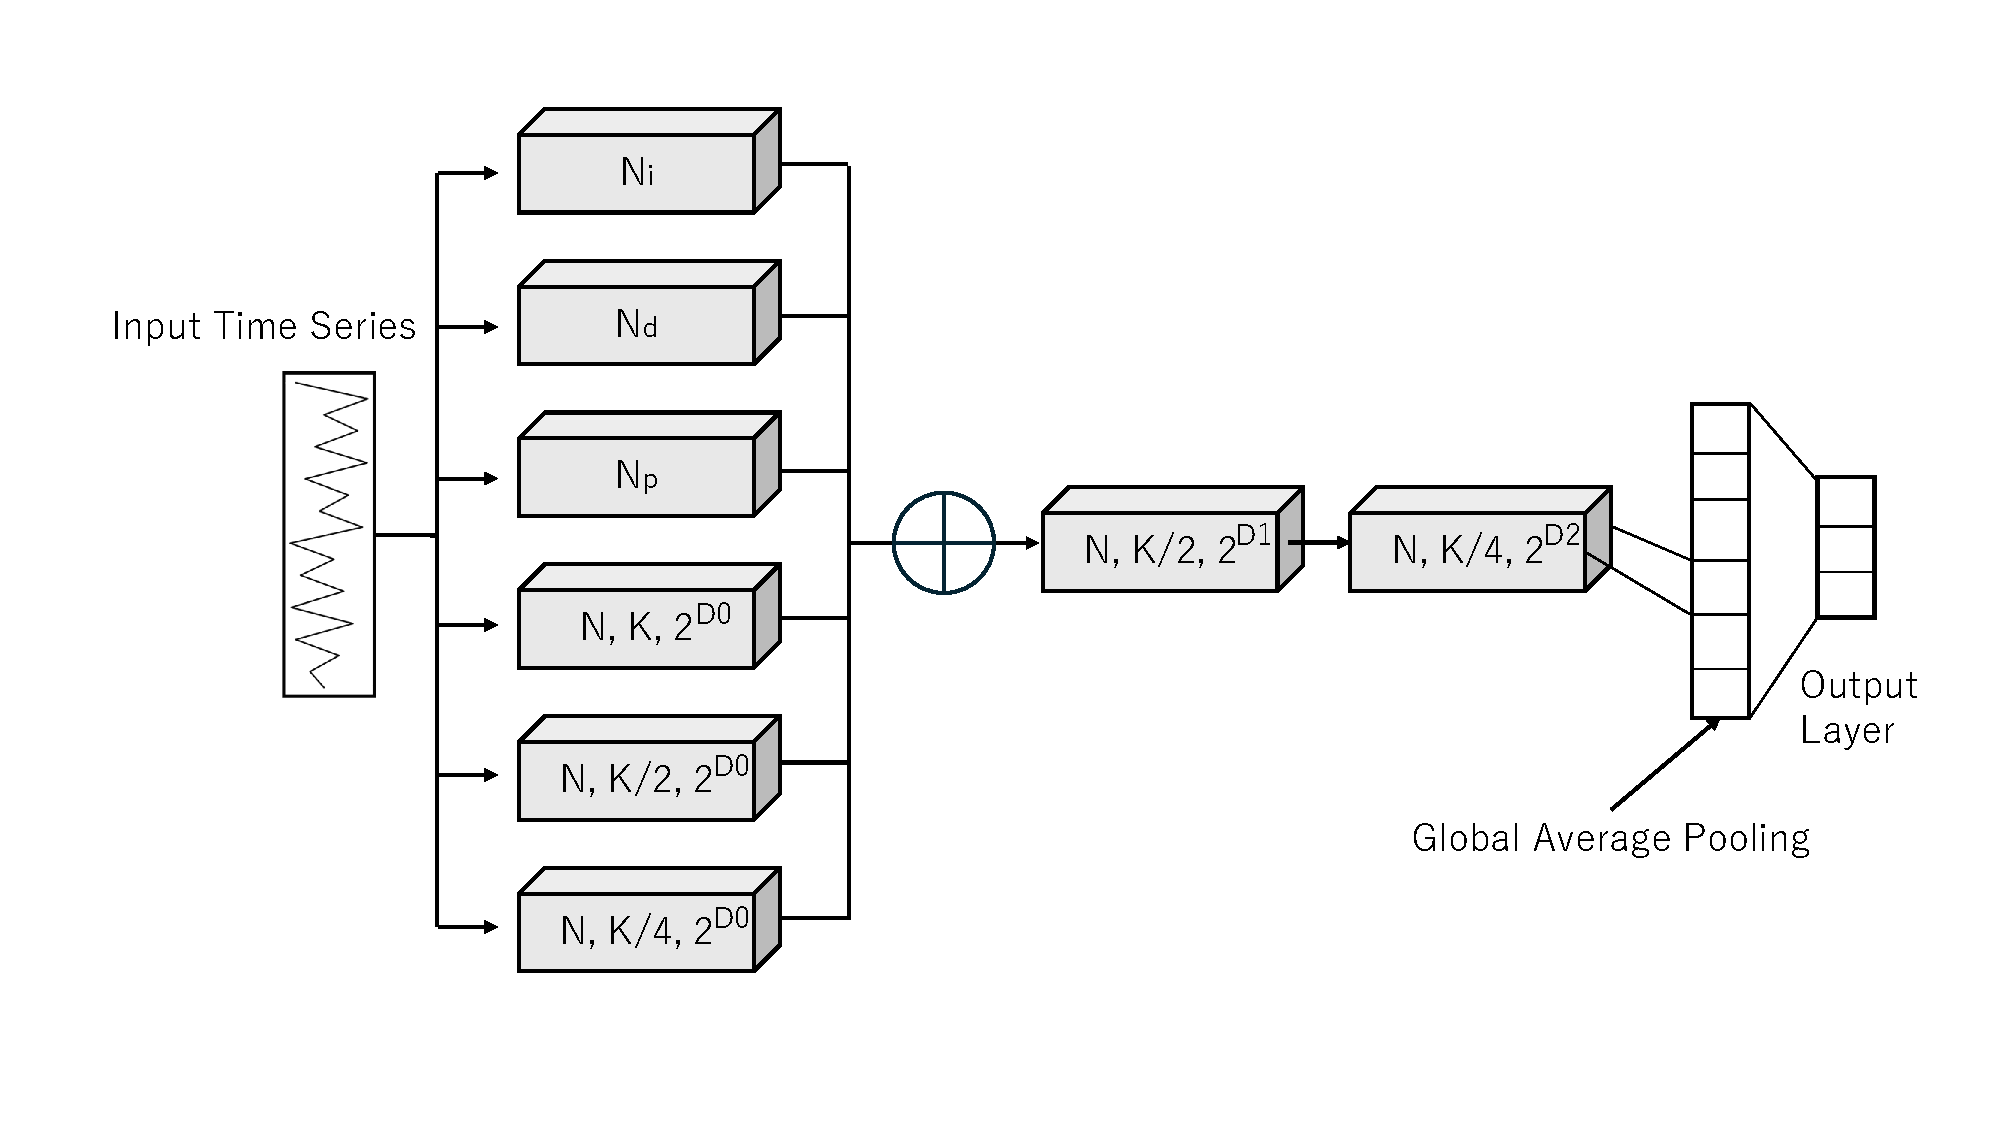
\includegraphics[width=\linewidth]{./fig/LITE_eng.pdf} 
  \caption{LITE Model}
  \label{fig:lite}
\end{figure}

\section{Proposed Model}

In this paper, we propose the modified version of LITE model; MC-MHLITE and PMC-MHLITE models.

\subsection{MC-MHLITE Model}

Figure \ref{fig:mc-mhlite} shows the structure of MC-MHLITE Model. In this model, there are three types of input data: the original time series data, and the short- and long-term MACD histograms. In this model, these data are composed as 3-dimensional multi-channel data. For the time series data $\mathbf{x}$, let the MACD histogram calculated using long-term parameters be denoted as $hist(\omega_{l_1}, \omega_{l_2}, \omega_{l_3})[\mathbf{x}]$, and the MACD histogram calculated using short-term parameters as $hist(\omega_{s_1},\omega_{s_2},\omega_{s_3})[\mathbf{x}]$. Here, the $i$th element of the 3-dimensional multi-channel data is
\begin{equation}
\begin{split}
multi3(\mathbf{x})_j = \langle &x_i, hist(\omega_{l_1},\omega_{l_2},\omega_{l_3})[\mathbf{x}]_i, \\
&hist(\omega_{s_1},\omega_{s_2},\omega_{s_3})[\mathbf{x}]_i \rangle.
\end{split}
\end{equation}
In this study, the parameters $\omega_{s_1}=3, \ \omega_{s_2}=5, \ and \ \omega_{s_3}=4$ are used to extract the short-term MACD and MACD histogram from the time series data. In addition, the long-term MACD and MACD histogram of time series data is extracted by using $\omega_{l_1}=13, \ \omega_{l_2}=26, \ and \ \omega_{l_3}=9$.


By incorporating the MACD histogram—which represents the acceleration of the time series data—into a multi-channel framework, weights are assigned to the features. Furthermore, the model emphasizes not only changes in the values of the time series data itself but also the simultaneous incorporation of the ``acceleration'' and trend changes of the time series data as represented by the MACD histograms. While the LITE model achieves lightweight performance by using depth-wise separable convolutions, accepting 3-dimensional multi-channel data as input enables it to learn both long-term fluctuation trends—which cannot be fully captured by a single time series—and short-term changes simultaneously. This emphasizes characteristic sub-time series and their changes, leading to an expected improvement in classification accuracy.


%本モデル（図\ref{fig:mc-mhlite}）は LITE に時系列データと MC-MHLF でも使用されていた時系列データから取り出した長短期 MACD ヒストグラムの 3 つを入力とするモデルである．時系列データの加速度を表現する MACD ヒストグラムを加えたマルチチャネルとすることで特徴に対する重み付けが行われる．また，時系列データそのものの値の変化だけでなく，MACD ヒストグラムによって表現される時系列データの「加速度」やトレンドの変化を同時に入力することに重点を置いている．LITE モデルは深さ単位分離可能畳み込みを用いることで軽量化を実現しているが，入力として 3 次元のマルチチャネルデータを受け取ることで，単一の時系列データだけでは捉えきれない長期的な変動傾向と，短期的な変化の両方を一度に学習させることが可能となる．これにより，特徴的な部分時系列データとその変化がより強調され，分類精度の向上が期待できる．


%ここで，時系列データ$\mathbf{x}$に対して，長期パラメータで算出したMACDヒストグラムを$hist(\omega_{l_1},\omega_{l_2},\omega_{l_3})[\mathbf{x}]$，短期パラメータで算出したMACDヒストグラムを$hist(\omega_{s_1},\omega_{s_2},\omega_{s_3})[\mathbf{x}]$とする．ここで，3次元のマルチチャネルデータの$i$番目の要素は
%$$
%multi3(\mathbf{x})_j = \langle x_i, hist(\omega_{l_1},\omega_{l_2},\omega_{l_3})[\mathbf{x}]_i, hist(\omega_{s_1},\omega_{s_2},\omega_{s_3})[\mathbf{x}]_i \rangle
%$$
%と定義される．

\begin{figure}[tb] 
  \centering
  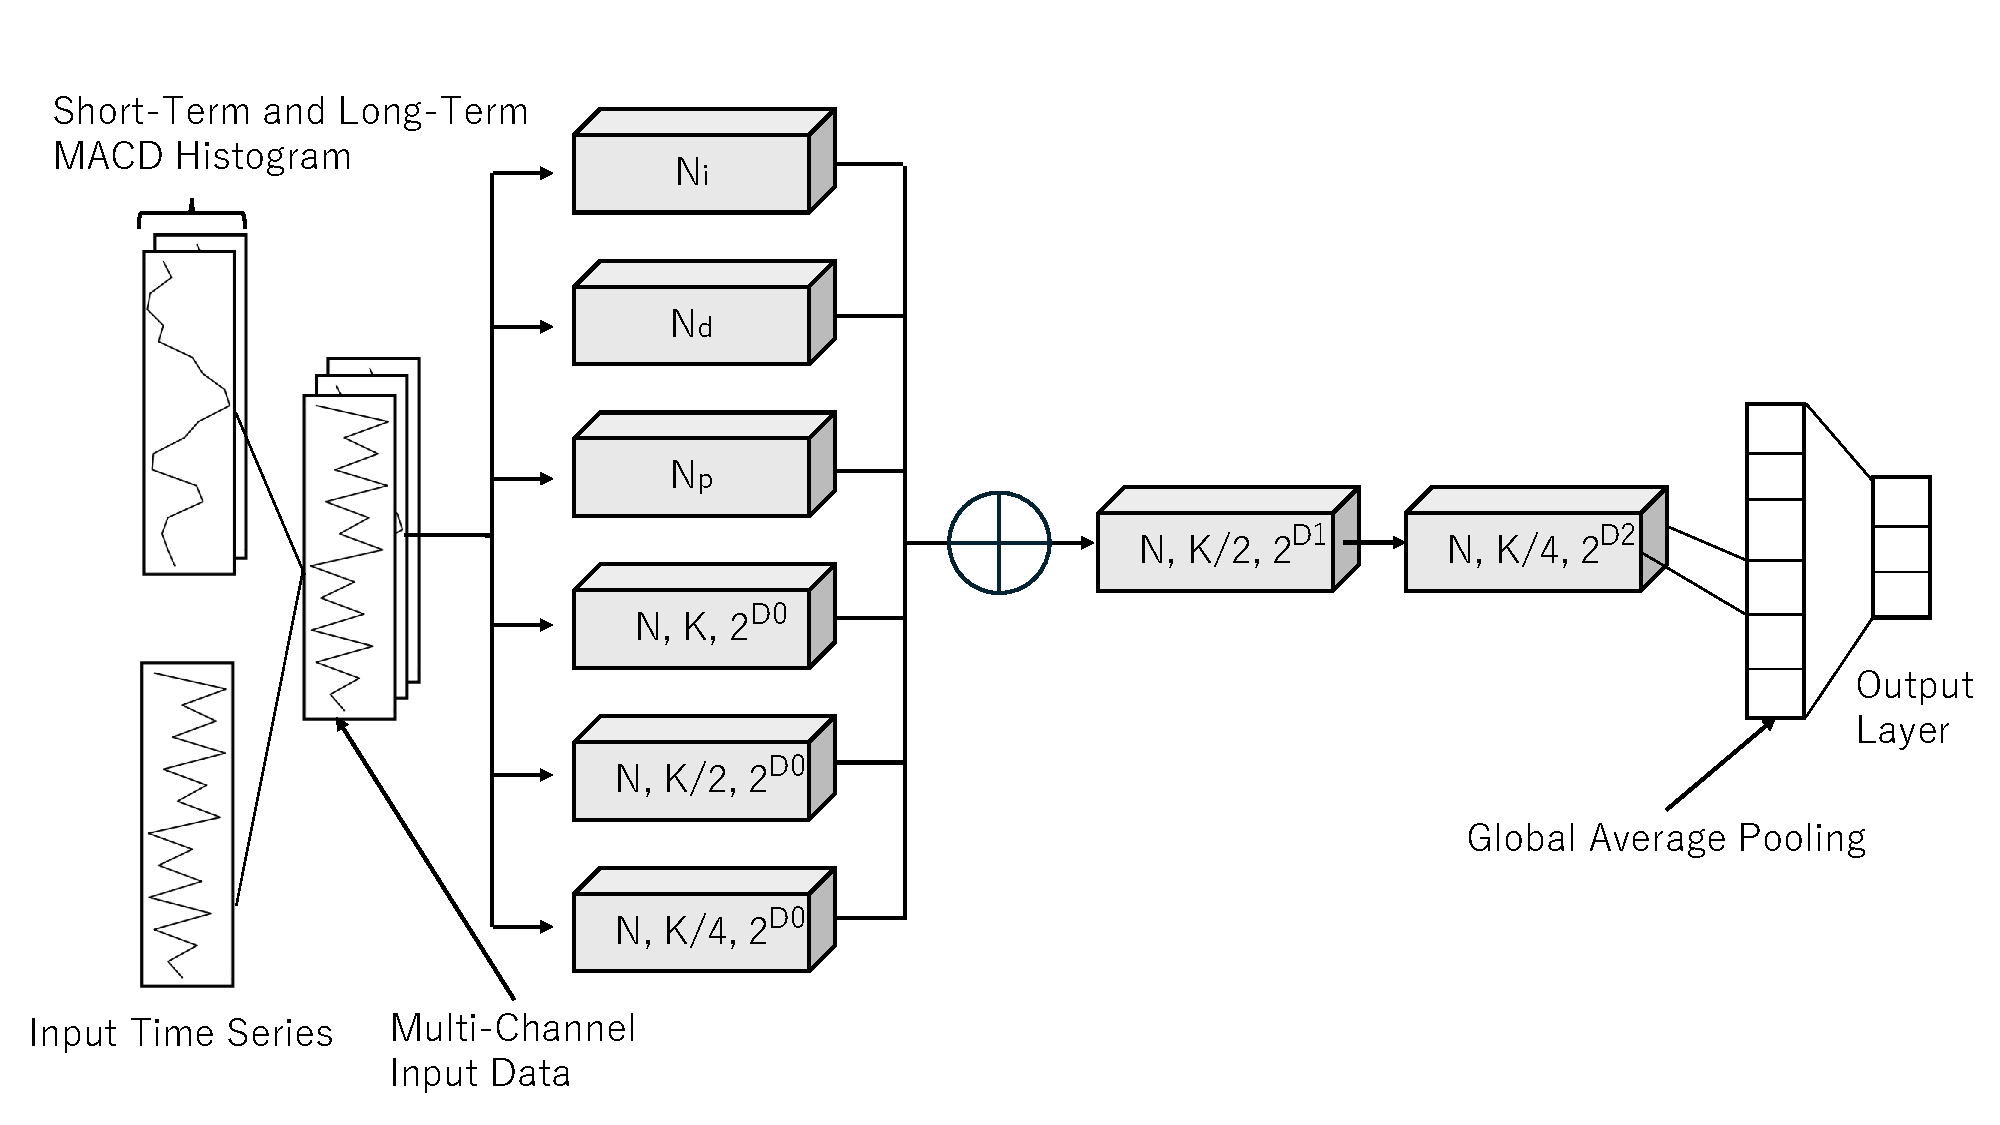
\includegraphics[width=\linewidth]{./fig/MC-MHLITE_eng.pdf} 
  \caption{MC-MHLITE Model}
  \label{fig:mc-mhlite}
\end{figure}

\subsection{PMC-MHLITE Model}

Figure \ref{fig:pmc-mhlite} shows the structure of PMC-MHLITE Model. This model consists of two LITE models running in parallel: one that takes time series data and a long-term MACD histogram as inputs, and another that takes time series data and a short-term MACD histogram as inputs. For the time series data $\mathbf{x}$, let the MACD histogram calculated using long-term parameters be denoted as $hist(\omega_{l_1}, \omega_{l_2}, \omega_{l_3})[\mathbf{x}]$, and the MACD histogram calculated using short-term parameters as $hist(\omega_{s_1},\omega_{s_2},\omega_{s_3})[\mathbf{x}]$. Here, the $i$th element of the two multi-channel data sets input to PMC-MHLITE is
\begin{equation}
lmulti2(\mathbf{x})_j = \langle x_i, hist(\omega_{l_1},\omega_{l_2},\omega_{l_3})[\mathbf{x}]_i \rangle
\end{equation}
\begin{equation}
smulti2(\mathbf{x})_j = \langle x_i, hist(\omega_{s_1},\omega_{s_2},\omega_{s_3})[\mathbf{x}]_i \rangle
\end{equation}

The outputs from the Global Average Pooling layers of these LITE models are combined in a fusion layer and fed into the output layer. By combining the long-term and short-term MACD histograms with the time series data to create a multi-channel input, the aim is to process different sub-time series data using separate LITE models, thereby extracting features from each dataset without compromising their distinct characteristics. Furthermore, since the LITE model itself is a lightweight model with a reduced number of parameters, even when two models are deployed in parallel, it is believed that high-precision classification utilizing more features is possible while keeping the increase in computational cost to a minimum.

%本モデル（図\ref{fig:pmc-mhlite}）は時系列データと長期 MACD ヒストグラムを入力とする LITE と時系列データと短期 MACD ヒストグラムを入力とするもう一つの LITE を並列に組み，LITE のGlobal Average Pooling 層の出力を結合層でで統合し，出力層につないだモデルである．長期と短期のMACD ヒストグラムを時系列データとマルチチャネル化させることで異なる部分時系列データを別々の LITE モデルで処理することで，互いのデータが持つ特徴を損なうことなく抽出することを狙いとしている．また，LITE モデル自体がパラメータ数を削減した軽量なモデルであるため，並列に2 つのモデルを配置しても，計算コストの大幅な増加を抑えつつ，より多くの特徴量を利用した高精度な分類が可能になると考えられる．

\begin{figure}[tb] 
  \centering
  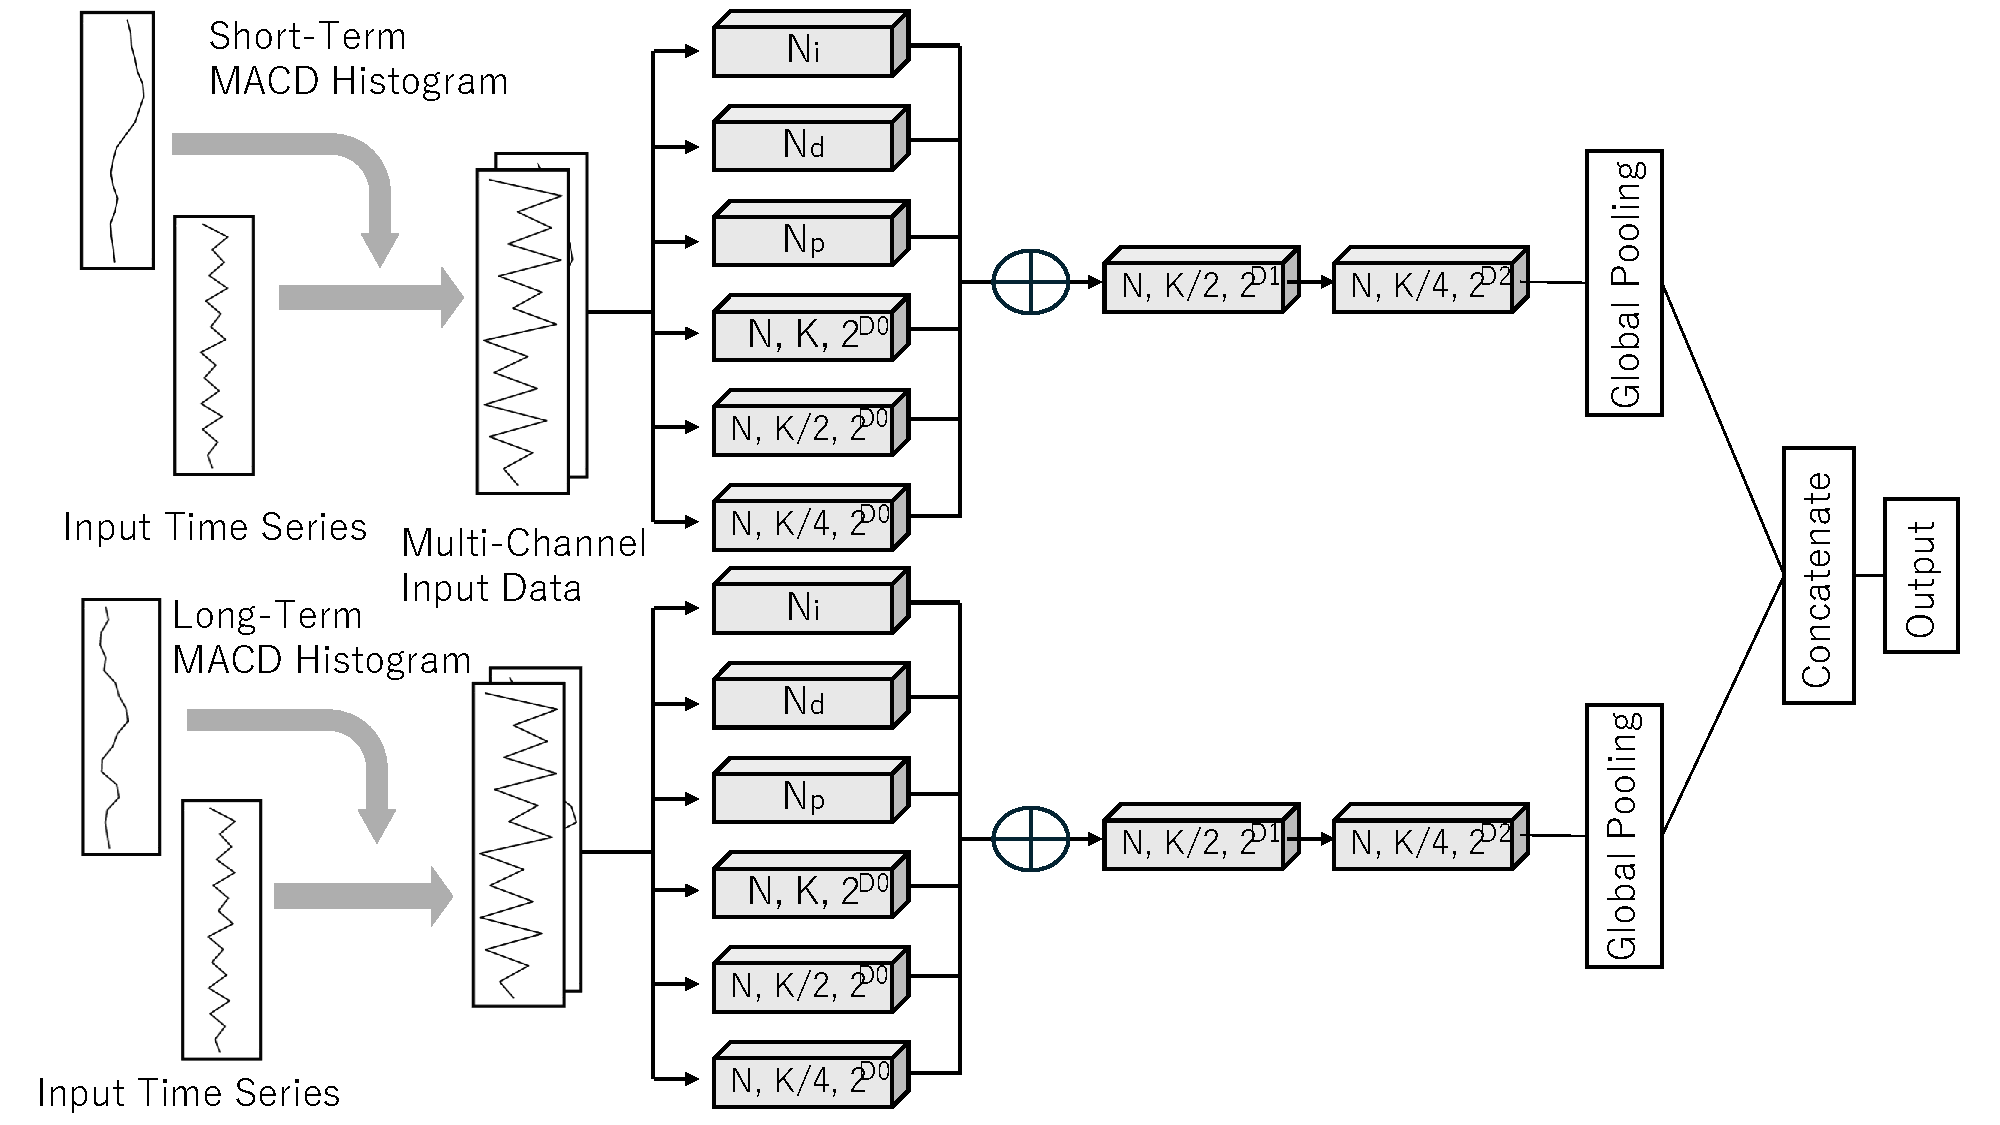
\includegraphics[width=\linewidth]{./fig/PMC-MHLITE_eng.pdf} 
  \caption{PMC-MHLITE Model}
  \label{fig:pmc-mhlite}
\end{figure}



%ここで，時系列データ$\mathbf{x}$に対して，長期パラメータで算出したMACDヒストグラムを$hist(\omega_{l_1},\omega_{l_2},\omega_{l_3})[\mathbf{x}]$，短期パラメータで算出したMACDヒストグラムを$hist(\omega_{s_1},\omega_{s_2},\omega_{s_3})[\mathbf{x}]$とする．ここで，PMC-MHLITEに入力する2つのマルチチャネルデータの$i$番目の要素は
%$$
%lmulti2(\mathbf{x})_j = \langle x_i, hist(\omega_{l_1},\omega_{l_2},\omega_{l_3})[\mathbf{x}]_i \rangle
%$$
%$$
%smulti2(\mathbf{x})_j = \langle x_i, hist(\omega_{s_1},\omega_{s_2},\omega_{s_3})[\mathbf{x}]_i \rangle
%$$
%と定義される．

\section{Experiments}

\subsection{Dataset}
In the experiments, we use the UCR Time Series Classification Archive released by the University of California, Riverside, which is widely used as a benchmark for time series classification. This archive consists of 85 datasets; each dataset contains time series data with varying lengths and has been pre-split into training and test datasets.

%本実験では，時系列分類のベンチマークとして広く利用されているカリフォルニア大学リバーサイド校公開の「UCRアーカイブデータセット」を使用する．本アーカイブは計85個のデータセットで構成されており，各データセットは異なる系列長を持つ時系列データを含み，あらかじめ訓練データとテストデータに分割されている．

These datasets are classified into the following seven categories based on their characteristics.

%これらのデータセットは，その特性に応じて以下の7つのカテゴリに分類される．
\begin{itemize}
    \item \textbf{Device}: Time series representing the states or usage patterns of electronic appliances and devices.
    \item \textbf{ECG}: Biometric signals captured via electrocardiography (ECG) to monitor cardiac activity.
    \item \textbf{Image}: Time series converted from image outlines or shapes.
    \item \textbf{Motion}: Data recording the physical movements and trajectories of human subjects or objects.
    \item \textbf{Sensor}: Physical measurements observed by environmental or industrial sensors.
    \item \textbf{Simulated}: Synthetic datasets generated through mathematical models or computational simulations.
    \item \textbf{Spectro}: Spectral data of substances (e.g., food or chemical compounds) acquired using a spectrometer.
\end{itemize}

\subsection{Criteria}
For each dataset, we trained the model using the training dataset and measured the accuracy using the test dataset. In the experiment, we compared classification accuracy, the number of parameters, and processing time with other models. The comparison models included the conventional MC-MHLF model and the LITE model. 

We evaluated the models using three metrics across all 85 datasets: average
accuracy, average of ranking, and number of best accuracy. The average accuracy
is the mean accuracy achieved for the test data across all 85 datasets. The
average of ranking is calculated by determining the ranking of the accuracy rates
among the models for each dataset, and then averaging these rankings across
the 85 datasets. The number of best accuracy is the number of datasets in which
a model achieved the highest accuracy rate, after determining the ranking of
accuracy rates among models for each dataset. 

\subsection{Environment}
Table \ref{tab:fcn_para} shows the parameters for each convolutional layer of the FCN and the number of units in LSTM was set to 128. 
The LITE architecture setup employs $N_i=6$ and $N_d=6$ (kernel sizes: $[2, 4, 8, 16, 32, 64]$), $N_p=5$ (kernel sizes: $[6, 12, 24, 48, 96]$), $N=32$, and $K=40$. Dilation rates are initialized at $D_0=1$ and incremented with network depth to $D_1=2$ and $D_2=4$.
Processing time was measured using a computer equipped with an NVIDIA GeForce RTX 4070 Ti (CPU: Intel(R) Core(TM) i7-4790 @ 3.60GHz, Memory: DDR3-1600 (PC3-12800) 16GB, Storage: 1TB WD Blue 3D NAND SATA WDS100T2B0A).


%%%%%%%%%%%%%%%%%%%%%%%%%%%%%%%%%%%%%%%%%%%%%%%%%%%%%%%%%%%%%%%%%%%%%
\begin{table}[tb]
\centering
\caption{MHLF's parameters}
\label{tab:fcn_para}
 \begin{tabular}{c|ccc} \hline \hline 
	   			&	Layer-1	&	Layer-2	&	Layer-3 	\\ \hline
Number of Filters		&	128	&	256	&	128		\\
Size of Kernel	&	8	&	5	&	3		\\ \hline
  \end{tabular}
\end{table}
%%%%%%%%%%%%%%%%%%%%%%%%%%%%%%%%%%%%%%%%%%%%%%%%%%%%%%%%%%%%%%%%%%%%


%実験では，他のモデルとの分類精度，パラメータ数，処理時間を比較した．比較モデルには従来手法の MC-MHLF モデルと LITE モデルを加えた．それら比較結果をカテゴリごとにまとめて表に示す．処理時間の測定は，NVIDIA 社の GPU，GeForce RTX 4070 Ti
%が搭載された計算機（CPU: Intel(R) Core(TM) i7-4790 CPU @ 3.60GHz，メモリ: DDR31600(PC3-12800) 16GB，ディスク: 1TB WD Blue 3D NAND SATA WDS100T2B0A）で行った．

\begin{table}[tb]
  \centering
  \caption{Summary of Comparison Results by Category}
  \label{tab:category_summary}
  \resizebox{\columnwidth}{!}{%
    \begin{tabular}{llccc}
      \toprule
      Category & Metric & LITE & MC-MHLITE & PMC-MHLITE \\
      \midrule
      \multirow{3}{*}{Device (6)} & Average of Accuracy & \textbf{0.735} & 0.728 & 0.725 \\
      & Average of Ranking & \textbf{1.500} & 2.167 & 2.333 \\
      & Number of Best Accuracy & \textbf{4} & 1 & 1 \\
      \midrule
      \multirow{3}{*}{ECG (6)} & Average of Accuracy & 0.960 & \textbf{0.963} & 0.961 \\
      & Average of Ranking & \textbf{1.667} & 1.833 & \textbf{1.667} \\
      & Number of Best Accuracy & \textbf{3} & 2 & \textbf{3} \\
      \midrule
      \multirow{3}{*}{Image (29)} & Average of Accuracy & 0.859 & 0.866 & \textbf{0.869} \\
      & Average of Ranking & 2.172 & \textbf{1.862} & \textbf{1.862} \\
      & Number of Best Accuracy & 10 & 10 & \textbf{11} \\
      \midrule
      \multirow{3}{*}{Motion (14)} & Average of Accuracy & 0.783 & 0.788 & \textbf{0.795} \\
      & Average of Ranking & 2.214 & 1.786 & \textbf{1.643} \\
      & Number of Best Accuracy & 4 & 5 & \textbf{7} \\
      \midrule
      \multirow{3}{*}{Sensor (18)} & Average of Accuracy & 0.862 & 0.861 & \textbf{0.869} \\
      & Average of Ranking & 1.778 & 2.056 & \textbf{1.333} \\
      & Number of Best Accuracy & 9 & 6 & \textbf{13} \\
      \midrule
      \multirow{3}{*}{Simulated (5)} & Average of Accuracy & 0.965 & 0.971 & \textbf{0.989} \\
      & Average of Ranking & \textbf{1.400} & 2.000 & \textbf{1.400} \\
      & Number of Best Accuracy & \textbf{4} & 2 & 3 \\
      \midrule
      \multirow{3}{*}{Spectro (7)} & Average of Accuracy & \textbf{0.900} & 0.886 & 0.897 \\
      & Average of Ranking & 1.571 & 2.286 & \textbf{1.429} \\
      & Number of Best Accuracy & \textbf{5} & 1 & \textbf{5} \\
      \midrule[1pt]
      \multirow{3}{*}{\textbf{Total Average}} & Average of Accuracy & 0.855 & 0.857 & \textbf{0.863} \\
      & Average of Ranking & 1.941 & 1.988 & \textbf{1.671} \\
      & Number of Best Accuracy & 38 & 26 & \textbf{43} \\
      \bottomrule
    \end{tabular}
  }
\end{table}


\subsection{Experiment 1}

Table \ref{tab:category_summary} shows the results of a performance comparison between the LITE model, the MC-MHLITE model, and the PMC-MHLITE model across seven categories.
Overall, the PMC-MHLITE model showed the best performance.The PMC-MHLITE model ranked first in all metrics, with the average of accuracy of 0.863, the average of ranking of 1.671, and the number of best accuracy of 43.  In particular, it performs well in categories with a large number of datasets, such as ``Image,'' ``Motion,'' and ``Sensor.'' In contrast, the LITE model is superior in a specific category. In particular, in ``Device'' category, the LITE model outperforms others with the average of ranking of 1.500 and the number of best accuracy of 4. This is because the Device category has data that is similar to spike signals or digital signals; therefore, it would be counter-productive to add a MACD histogram. The MC-MHLITE model showed good accuracy only in ``ECG,'' but the number of best accuracy was achieved in only 26 datasets. The average rank was also the lowest. In conclusion, the PMC-MHLITE model is the best for a wide range of datasets. However, it is also necessary to select a model according to the characteristics of the target category.

%全体として，PMC-MHLITEモデルが最も優れた汎用性を示した．PMC-MHLITEモデルは平均精度0.863，平均順位1.671，最高精度の獲得数43と，すべての指標で首位を記録した．特にImage，Motion，Sensorといったデータセット数が多いカテゴリで性能がよい．
%
%一方で，LITEモデルが特定のカテゴリで優位に立つ．特にDeviceカテゴリでは，LITEが平均順位1.500，最高精度獲得数4と他を大きく引き離した．Deviceカテゴリのデータはスパイク信号やデジタル信号に近いデータがありMACDヒストグラムを加えると逆効果であることが理由としてあげられる．MC-MHLITEモデルは，ECGなどの特定のカテゴリで良好な精度を示しているが，最高精度獲得数は26件に留まった．平均順位も最下位であった．
%
%結論として，広範なタスクで高い安定性を求めるならばPMC-MHLITEモデルが最適である．ただし，DeviceデータのようにLITEが優位なカテゴリも存在するため，対象の特性に応じたモデル選択も必要である．



%%表\ref{tab:category_summary}は，7つのカテゴリごとにLITEモデル，MC-MHLITEモデル，およびPMC-MHLITEモデルの性能を比較した結果である．
%
%The PMC-MHLITE model achieved the highest average of ranking and number of best accuracy results in five out of the seven categories. In particular, it achieved stable accuracy comparable to the LITE model in categories with relatively large datasets, such as ``Image,'' ``Motion,'' and ``Sensor.'' This is believed to be the result of more accurately capturing the dynamic changes in time series data by separately converting the long-term and short-term MACD histograms into multiple channels and training them in parallel.
%
%%PMC-MHLITEモデルの性能は，全7カテゴリのうち``Device''を除く6カテゴリにおいて，平均ランクおよび最高精度数でトップの数値となった．特に``Image''や``Motion''，``Sensor''といった比較的データセット数が多いカテゴリにおいて，LITEモデルと安定した精度を達成している．これは，長短期のMACDヒストグラムを個別にマルチチャネル化し並列に学習させることで，時系列データの動的な変化をより正確に捉えられた結果であると考えられる．
%
%On the other hand, in the ``Device'' category, the LITE model achieved an average accuracy of 0.735 and an Average of Ranking of 1.667, outperforming the proposed model. The datasets included in ``Device'' (such as power consumption) tend to emphasize periodicity and the presence of specific patterns, suggesting that the addition of acceleration information via the MACD histogram does not necessarily work effectively in all domains.
%
%%一方で，``Device''カテゴリにおいては，LITEモデルが平均正解率0.735，平均ランク1.667となり，提案モデルを上回る結果となった．``Device''に含まれるデータセット（電力使用量など）は，周期性や特定のパターンの有無が重視される傾向にあり，MACDヒストグラムによる加速度情報の付与が，必ずしもすべてのドメインで有効に機能するわけではないことを示唆している．
%
%%The PMC-MHLITE model achieved an average accuracy of 0.863 and an average of ranking of 1.671, demonstrating an improvement over the LITE model (average accuracy of 0.855, Average of Ranking of 2.224). 
%%In terms of the number of instances with the highest accuracy, the PMC-MHLITE model achieved the highest accuracy on approximately 45 instances as the LITE model (24 instances), demonstrating that the proposed method is a highly versatile model.
%
%%しかし，全体をみると，PMC-MHLITEモデルは平均正解率0.863，平均ランク1.629を達成し，LITEモデル（平均正解率0.855，平均ランク2.224）に対して改善を果たすことができている．最高精度数においても，LITEモデルの24件に対しPMC-MHLITEモデルは45件と約2倍のデータセットで最高精度となり，提案手法が汎用性の高いモデルであることが示された．

\begin{figure}[tb] 
  \centering
  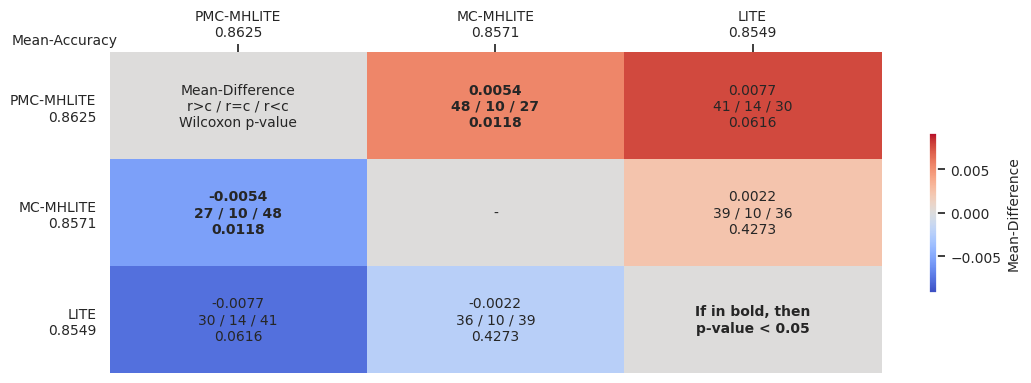
\includegraphics[width=\linewidth]{./fig/MCM.png} 
  \caption{Multi Comparison Matrix}
  \label{fig:Multi Comparison Matrix}
\end{figure}

\subsection{Evaluation Experiment 2}

\begin{table}[tb]
  \centering
  \caption{Summary of Comparison Results by Category (Including MC-MHLF)}
  \label{tab:category_summary_updated}
  \resizebox{\columnwidth}{!}{%
    \begin{tabular}{llcccc}
      \toprule
      Category & Metric & MC-MHLF & LITE & MC-MHLITE & PMC-MHLITE \\
      \midrule
      \multirow{3}{*}{Device (6)} & Average of Accuracy & \textbf{0.755} & 0.735 & 0.728 & 0.725 \\
      & Average of Ranking & \textbf{1.167} & 2.333 & 3.167 & 3.333 \\
      & Number of Best Accuracy & \textbf{5} & 1 & 0 & 0 \\
      \midrule
      \multirow{3}{*}{ECG (6)} & Average of Accuracy & \textbf{0.968} & 0.960 & 0.963 & 0.961 \\
      & Average of Ranking & \textbf{1.000} & 2.333 & 2.500 & 2.500 \\
      & Number of Best Accuracy & \textbf{6} & 2 & 2 & 1 \\
      \midrule
      \multirow{3}{*}{Image (29)} & Average of Accuracy & \textbf{0.887} & 0.859 & 0.866 & 0.869 \\
      & Average of Ranking & \textbf{1.379} & 3.034 & 2.586 & 2.724 \\
      & Number of Best Accuracy & \textbf{22} & 4 & 3 & 2 \\
      \midrule
      \multirow{3}{*}{Motion (14)} & Average of Accuracy & \textbf{0.806} & 0.783 & 0.788 & 0.795 \\
      & Average of Ranking & \textbf{1.857} & 2.857 & 2.429 & 2.071 \\
      & Number of Best Accuracy & \textbf{7} & 4 & 3 & 4 \\
      \midrule
      \multirow{3}{*}{Sensor (18)} & Average of Accuracy & \textbf{0.878} & 0.862 & 0.861 & 0.869 \\
      & Average of Ranking & 2.000 & 2.222 & 2.556 & \textbf{1.833} \\
      & Number of Best Accuracy & \textbf{11} & 6 & 4 & 9 \\
      \midrule
      \multirow{3}{*}{Simulated (5)} & Average of Accuracy & \textbf{0.991} & 0.965 & 0.971 & 0.989 \\
      & Average of Ranking & 2.000 & 1.800 & 2.600 & \textbf{1.600} \\
      & Number of Best Accuracy & \textbf{3} & \textbf{3} & 2 & \textbf{3} \\
      \midrule
      \multirow{3}{*}{Spectro (7)} & Average of Accuracy & \textbf{0.941} & 0.900 & 0.886 & 0.897 \\
      & Average of Ranking & \textbf{1.286} & 2.000 & 3.143 & 2.000 \\
      & Number of Best Accuracy & \textbf{5} & 4 & 1 & 3 \\
      \midrule[1pt]
      \multirow{3}{*}{\textbf{Total Average (85)}} & Average of Accuracy & \textbf{0.879} & 0.855 & 0.857 & 0.863 \\
      & Average of Ranking & \textbf{1.576} & 2.612 & 2.682 & 2.341 \\
      & Number of Best Accuracy & \textbf{59} & 23 & 14 & 21 \\
	& Processing Time [s] & 1895.194 & \textbf{995.820} & 1020.266 & 1421.505 \\
      & Number of Parameters & 273,619 & \textbf{10,859} & 16,215 & 27,067 \\
      \bottomrule
    \end{tabular}
  }
\end{table}


Table \ref{tab:category_summary_updated} provides a comprehensive comparison of the performance of each model across all 85 datasets.  We discuss the trade-off between the effectiveness and computational cost of the proposed model based on these results.

%表\ref{table:comparison_results}は，全85データセットにおける各モデルの性能を総合的に比較したものである．本結果に基づき，提案モデルの有効性と計算コストのトレードオフについて考察する．

First, in terms of accuracy, the MC-MHLF model recorded an average correct rate of 0.879 and an average of ranking of 1.576, demonstrating the best performance among the four models. However, the MC-MHLF model has a notably high number of parameters—approximately 274,000—and the longest average processing time at 1,895.194 seconds. In contrast, the MC-MHLITE model, which was designed to be more lightweight, reduced the number of parameters to approximately one-seventeenth (16,215) of that of the MC-MHLF model, while still achieving an average accuracy of 0.857, surpassing the baseline LITE model (0.855).

%まず，精度の観点ではMC-MHLFモデルが平均正解率0.879，平均ランク1.576を記録し，4つのモデル中で最高のパフォーマンスを示した．しかし，MC-MHLFモデルのパラメータ数は約27.4万個と突出しており，平均処理時間も1895.194秒と最も長い．これに対し，軽量化を図ったMC-MHLITEモデルは，パラメータ数をMC-MHLFモデルの約17分の1（16,215個）に削減しながらも，ベースラインであるLITEモデル（0.855）を上回る0.857の平均正解率を達成している．

Furthermore, focusing on the PMC-MHLITE model, the average accuracy improved to 0.863, and the average of ranking also improved to 2.341. Although the number of parameters has increased slightly to 27,066, it remains about one-tenth the size of the MC-MHLF model. In terms of processing time, while the MC-MHLF model takes approximately 1,900 seconds, the PMC-MHLITE model takes about 1,422 seconds, achieving a reduction of approximately 25\%.

%さらに，PMC-MHLITEモデルに注目すると，平均正解率は0.863まで向上し，平均ランクも2.341へと改善された．パラメータ数は27,066個と微増しているものの，MC-MHLFモデルの約10分の1の規模に留まっている．処理時間についても，MC-MHLFモデルが約1900秒を要するのに対し，PMC-MHLITEモデルは約1422秒と約25\%の短縮を実現している．


%\subsection{Evaluation Experiment 3}
%
%Table \ref{tab:comparison_costs} shows the results of comparing the model training and inference times for the MC-MHLF, LITE, MC-MHLITE, and PMC-MHLITE models using datasets selected for each category.
%
%%表\ref{tab:comparison_costs}は，各カテゴリごとに選定したデータセットでMC-MHLF，LITEモデル，MC-MHLITEモデル，およびPMC-MHLITEモデルのモデル学習処理時間と推論処理時間を比較した結果である．
%
%Since the processing times were generally not very long, although some errors may have occurred, the results generally aligned with the number of model parameters.
%
%%全体的に処理時間の値が大きくないため，誤差は起きうるが概ねモデルパラメータ数に沿う結果となった。

%\begin{table}[tb]
%  \centering
%  \caption{Comparison of Computational Costs Across Models}
%  \label{tab:comparison_costs}
%  \resizebox{\columnwidth}{!}{%
%    \begin{tabular}{llcccc}
%      \toprule
%      Dataset & Metric & MC-MHLF & LITE & MC-MHLITE & PMC-MHLITE \\
%      \midrule
%      \multirow{2}{*}{Adiac} & Average learning time [s] & 1608 & \textbf{1062} & 1075 & 1561 \\
%      & Average inference time [s] & 0.067 & \textbf{0.060} & 0.061 & 0.069 \\
%      \midrule
%      \multirow{2}{*}{CBF} & Average learning time [s] & 753 & \textbf{667} & 675 & 873 \\
%      & Average inference time [s] & 0.078 & \textbf{0.068} & 0.072 & 0.084 \\
%      \midrule
%      \multirow{2}{*}{Coffee} & Average learning time [s] & \textbf{385} & 398 & 400 & 511 \\
%      & Average inference time [s] & 0.053 & \textbf{0.051} & 0.052 & 0.057 \\
%      \midrule
%      \multirow{2}{*}{Computers} & Average learning time [s] & 567 & \textbf{403} & 427 & 595 \\
%      & Average inference time [s] & 0.081 & \textbf{0.058} & 0.064 & 0.074 \\
%      \midrule
%      \multirow{2}{*}{ECG200} & Average learning time [s] & \textbf{341} & 388 & 389 & 483 \\
%      & Average inference time [s] & 0.052 & \textbf{0.050} & 0.051 & 0.058 \\
%      \midrule
%      \multirow{2}{*}{Gun\_Point} & Average learning time [s] & 523 & 501 & \textbf{461} & 667 \\
%      & Average inference time [s] & 0.059 & \textbf{0.054} & 0.056 & 0.061 \\
%      \midrule
%      \multirow{2}{*}{wafer} & Average learning time [s] & 8813 & \textbf{5441} & 5816 & 7830 \\
%      & Average inference time [s] & 0.245 & \textbf{0.143} & 0.162 & 0.234 \\
%      \bottomrule
%    \end{tabular}
%  }
%\end{table}

\section{Conclusion}
In this paper, we proposed the MC-MHLITE and PMC-MHLITE models to achieve both high accuracy and lightweight performance for TSC. These models integrate MACD histograms, which  capture dynamic changes in time series, into the LITE model. By introducing short- and long-term MACD histograms that represent the acceleration of time series data, we enabled the efficient learning of trend changes that are difficult to extract from a single time series alone. The experimental results show that the PMC-MHLITE model is the best overall performance compared with the LITE and MC-MHLITE models. Compared to the MC-MHLF model, the PMC-MHLITE model is about one-tenth the size in parameters and 25\% faster in processing time. In our future work, we will develop more accurate lightweight models based on our approaches. We succeeded in reducing parameters, but the effect of processing time reduction was small due to library problems in implementation. We are going to address implementation issues and speed up the process.

%In this paper, with the aim of achieving both high accuracy and lightweight performance in TSC, we propose the MC-MHLITE and PMC-MHLITE models, which integrate the MACD histogram—designed to capture dynamic changes in time series—into the lightweight LITE model, which utilizes depth-wise separable convolutions. By introducing short- and long-term MACD histograms that represent the acceleration of time series data, we enabled the efficient learning of trend changes that are difficult to extract from a single time series alone.

%本論文では，TSCにおける高精度化と軽量化の両立を目的とし，深さ単位分離可能畳み込みを用いた軽量モデルLITEに，時系列の動的変化を捉えるMACDヒストグラムを統合した MC-MHLITEモデルおよびPMC-MHLITEモデルを提案した．時系列データの加速度を表現する長短期のMACDヒストグラムを導入することで，単一の系列データのみでは抽出が困難なトレンドの変化を効率的に学習可能とした．

\section{Acknowledgments}
This work was supported by JSPS KAKENHI Grant Number 23K11340. The authors wish to acknowledge Professor Eamonn Keogh and all those who contributed to the creation of the UCR time series classification archive.


\bibliographystyle{IEEEtran}

\appendices


\section{Detailed Comparison of Classification Accuracy}

This appendix provides a comprehensive evaluation of classification accuracy across 85 datasets from the UCR Time Series Archive, categorized into seven major domains as shown in Table \ref{tab:device_results} (Device), Table \ref{tab:ecg_accuracy} (ECG), Table \ref{tab:image_accuracy} (Image), Table \ref{tab:motion_accuracy} (Motion), Table \ref{tab:sensor_accuracy} (Sensor), Table \ref{tab:simulated_accuracy} (Simulated), and Table \ref{tab:spectro_accuracy} (Spectro). The performance of four models: MC-MHLF, LITE, MC-MHLITE, and PMC-MHLITE models, is compared based on average accuracy, average ranking, and the number of best accuracy results.
\bibliography{related}

\begin{table}[htb]
  \centering
  \caption{Comparison of classification accuracy for each model in the ``Device'' category}
  \label{tab:device_results}
  \resizebox{\columnwidth}{!}{%
    \begin{tabular}{lcccc}
      \toprule
      Dataset & MC-MHLF & LITE & MC-MHLITE & PMC-MHLITE \\
      \midrule
      Computers & 0.816 & \textbf{0.824} & 0.784 & 0.792 \\
      ElectricDevices & \textbf{0.761} & 0.714 & 0.707 & 0.712 \\
      \makecell[l]{LargeKitchen\\Appliances} & \textbf{0.912} & 0.891 & 0.888 & 0.877 \\
      \makecell[l]{Refrigeration\\Devices} & \textbf{0.589} & 0.576 & 0.579 & 0.587 \\
      ScreenType & \textbf{0.621} & 0.603 & 0.616 & 0.595 \\
      \makecell[l]{SmallKitchen\\Appliances} & \textbf{0.832} & 0.800 & 0.792 & 0.784 \\
      \midrule
      Average of Accuracy & \textbf{0.755} & 0.735 & 0.728 & 0.724 \\
      Average of Ranking & \textbf{1.167} & 2.333 & 3.167 & 3.333 \\
      Number of Best Accuracy & \textbf{5} & 1 & 0 & 0 \\
      \bottomrule
    \end{tabular}
  }
\end{table}

\begin{table}[htb]
  \centering
  \caption{Comparison of classification accuracy for each model in the ``ECG'' category}
  \label{tab:ecg_accuracy}
  \resizebox{\columnwidth}{!}{%
    \begin{tabular}{lcccc}
      \toprule
      Dataset & MC-MHLF & LITE & MC-MHLITE & PMC-MHLITE \\
      \midrule
      ECG200 & \textbf{0.930} & 0.910 & \textbf{0.930} & 0.910 \\
      ECG5000 & \textbf{0.948} & \textbf{0.948} & 0.946 & 0.945 \\
      ECGFiveDays & \textbf{1.000} & \textbf{1.000} & \textbf{1.000} & \textbf{1.000} \\
      \makecell[l]{NonInvasiveFatal\\ECG\_Thorax1} & \textbf{0.962} & 0.950 & 0.957 & 0.960 \\
      \makecell[l]{NonInvasiveFatal\\ECG\_Thorax2} & \textbf{0.965} & 0.955 & 0.950 & 0.953 \\
      TwoLeadECG & \textbf{1.000} & 0.997 & 0.997 & 0.999 \\
      \midrule
      Average of Accuracy & \textbf{0.968} & 0.960 & 0.963 & 0.961 \\
      Average of Ranking & \textbf{1.000} & 2.333 & 2.500 & 2.500 \\
      Number of Best Accuracy & \textbf{6} & 2 & 2 & 1 \\
      \bottomrule
    \end{tabular}
  }
\end{table}

\begin{table}[htb]
  \centering
  \caption{Comparison of classification accuracy for each model in the ``Image'' category}
  \label{tab:image_accuracy}
  \resizebox{\columnwidth}{!}{%
    \begin{tabular}{lcccc}
      \toprule
      Dataset & MC-MHLF & LITE & MC-MHLITE & PMC-MHLITE \\
      \midrule
      50words & \textbf{0.820} & 0.745 & 0.787 & 0.778 \\
      Adiac & \textbf{0.867} & 0.801 & 0.818 & 0.857 \\
      ArrowHead & \textbf{0.909} & 0.777 & 0.823 & 0.829 \\
      BeetleFly & \textbf{1.000} & 0.950 & \textbf{1.000} & 0.950 \\
      BirdChicken & 0.950 & \textbf{1.000} & 0.950 & \textbf{1.000} \\
      \makecell[l]{DiatomSize\\Reduction} & \textbf{0.980} & 0.958 & 0.931 & 0.961 \\
      \makecell[l]{DistalPhalanx\\OutlineAgeGroup} & \textbf{0.863} & 0.835 & 0.845 & 0.808 \\
      \makecell[l]{DistalPhalanx\\OutlineCorrect} & \textbf{0.843} & 0.818 & 0.812 & 0.817 \\
      DistalPhalanxTW & \textbf{0.808} & 0.775 & 0.793 & 0.790 \\
      FaceAll & \textbf{0.968} & 0.856 & 0.921 & 0.927 \\
      FaceFour & \textbf{0.989} & 0.955 & 0.920 & 0.943 \\
      FacesUCR & 0.961 & 0.960 & \textbf{0.963} & 0.961 \\
      FISH & 0.994 & 0.989 & 0.994 & \textbf{1.000} \\
      HandOutlines & 0.883 & \textbf{0.914} & 0.892 & 0.890 \\
      Herring & 0.750 & \textbf{0.766} & 0.750 & 0.734 \\
      MedicalImages & \textbf{0.782} & 0.775 & 0.758 & 0.771 \\
      \makecell[l]{MiddlePhalanx\\OutlineAgeGroup} & \textbf{0.813} & 0.788 & 0.783 & 0.775 \\
      \makecell[l]{MiddlePhalanx\\OutlineCorrect} & \textbf{0.848} & 0.810 & 0.838 & 0.822 \\
      MiddlePhalanxTW & \textbf{0.647} & 0.639 & 0.627 & 0.629 \\
      OSULeaf & \textbf{1.000} & 0.950 & 0.996 & 0.992 \\
      \makecell[l]{Phalanges\\OutlinesCorrect} & \textbf{0.848} & 0.843 & 0.845 & 0.846 \\
      \makecell[l]{ProximalPhalanx\\OutlineAgeGroup} & 0.883 & 0.878 & \textbf{0.888} & 0.873 \\
      \makecell[l]{ProximalPhalanx\\OutlineCorrect} & \textbf{0.931} & 0.921 & 0.914 & 0.911 \\
      ProximalPhalanxTW & 0.817 & \textbf{0.827} & 0.825 & 0.815 \\
      ShapesAll & \textbf{0.943} & 0.888 & 0.900 & 0.937 \\
      SwedishLeaf & \textbf{0.989} & 0.960 & 0.971 & 0.968 \\
      Symbols & \textbf{0.981} & 0.963 & 0.972 & 0.972 \\
      WordsSynonyms & \textbf{0.724} & 0.655 & 0.683 & 0.716 \\
      yoga & \textbf{0.935} & 0.907 & 0.912 & 0.924 \\
      \midrule
      Average of Accuracy & \textbf{0.887} & 0.859 & 0.866 & 0.869 \\
      Average of Ranking & \textbf{1.379} & 3.034 & 2.586 & 2.724 \\
      Number of Best Accuracy & \textbf{22} & 4 & 3 & 2 \\
      \bottomrule
    \end{tabular}
  }
\end{table}

\begin{table}[htb]
  \centering
  \caption{Comparison of classification accuracy for each model in the ``Motion'' category}
  \label{tab:motion_accuracy}
  \resizebox{\columnwidth}{!}{%
    \begin{tabular}{lcccc}
      \toprule
      Dataset & MC-MHLF & LITE & MC-MHLITE & PMC-MHLITE \\
      \midrule
      Cricket\_X & 0.815 & \textbf{0.821} & 0.787 & 0.818 \\
      Cricket\_Y & 0.831 & \textbf{0.862} & 0.815 & 0.831 \\
      Cricket\_Z & 0.869 & 0.841 & 0.841 & \textbf{0.877} \\
      Gun\_Point & \textbf{1.000} & \textbf{1.000} & \textbf{1.000} & \textbf{1.000} \\
      Haptics & 0.591 & 0.565 & \textbf{0.604} & 0.591 \\
      InlineSkate & \textbf{0.487} & 0.422 & 0.465 & 0.471 \\
      ToeSegmentation1 & \textbf{0.982} & \textbf{0.982} & 0.969 & 0.965 \\
      ToeSegmentation2 & \textbf{0.962} & 0.923 & 0.938 & 0.915 \\
      \makecell[l]{uWaveGesture\\Library\_X} & 0.819 & 0.812 & \textbf{0.833} & 0.831 \\
      \makecell[l]{uWaveGesture\\Library\_Y} & 0.733 & 0.716 & 0.741 & \textbf{0.743} \\
      \makecell[l]{uWaveGesture\\Library\_Z} & \textbf{0.775} & 0.756 & 0.772 & 0.764 \\
      \makecell[l]{uWaveGesture\\LibraryAll} & 0.895 & 0.900 & 0.905 & \textbf{0.911} \\
      Worms & \textbf{0.735} & 0.591 & 0.591 & 0.635 \\
      WormsTwoClass & \textbf{0.796} & 0.768 & 0.773 & 0.779 \\
      \midrule
      Average of Accuracy & \textbf{0.806} & 0.783 & 0.788 & 0.795 \\
      Average of Ranking & \textbf{1.857} & 2.857 & 2.429 & 2.071 \\
      Number of Best Accuracy & \textbf{7} & 4 & 3 & 4 \\
      \bottomrule
    \end{tabular}
  }
\end{table}

\begin{table}[htb]
  \centering
  \caption{Comparison of classification accuracy for each model in the ``Sensor'' category}
  \label{tab:sensor_accuracy}
  \resizebox{\columnwidth}{!}{%
    \begin{tabular}{lcccc}
      \toprule
      Dataset & MC-MHLF & LITE & MC-MHLITE & PMC-MHLITE \\
      \midrule
      Car & \textbf{0.933} & \textbf{0.933} & 0.883 & 0.900 \\
      \makecell[l]{Chlorine\\Concentration} & 0.816 & \textbf{0.826} & 0.823 & 0.813 \\
      CinC\_ECG\_torso & 0.903 & 0.871 & 0.946 & \textbf{0.959} \\
      Earthquakes & \textbf{0.826} & 0.823 & 0.820 & 0.823 \\
      FordA & 0.933 & 0.951 & \textbf{0.955} & \textbf{0.955} \\
      FordB & 0.929 & 0.934 & 0.934 & \textbf{0.939} \\
      \makecell[l]{InsectWingbeat\\Sound} & 0.584 & 0.605 & 0.625 & \textbf{0.633} \\
      \makecell[l]{ItalyPower\\Demand} & 0.968 & \textbf{0.970} & 0.959 & \textbf{0.970} \\
      Lighting2 & \textbf{0.885} & 0.820 & 0.836 & 0.836 \\
      Lighting7 & \textbf{0.877} & 0.822 & 0.795 & 0.849 \\
      MoteStrain & \textbf{0.895} & 0.886 & 0.855 & 0.872 \\
      Phoneme & \textbf{0.363} & 0.309 & 0.306 & 0.328 \\
      Plane & \textbf{1.000} & \textbf{1.000} & \textbf{1.000} & \textbf{1.000} \\
      \makecell[l]{SonyAIBORobot\\Surface} & \textbf{0.982} & 0.845 & 0.885 & 0.870 \\
      \makecell[l]{SonyAIBORobot\\SurfaceII} & \textbf{0.940} & 0.937 & 0.903 & 0.920 \\
      StarLightCurves & 0.967 & 0.979 & 0.979 & \textbf{0.980} \\
      Trace & \textbf{1.000} & \textbf{1.000} & \textbf{1.000} & \textbf{1.000} \\
      wafer & \textbf{0.999} & \textbf{0.999} & \textbf{0.999} & \textbf{0.999} \\
      \midrule
      Average of Accuracy & \textbf{0.878} & 0.862 & 0.861 & 0.869 \\
      Average of Ranking & 2.000 & 2.222 & 2.556 & \textbf{1.833} \\
      Number of Best Accuracy & \textbf{11} & 6 & 4 & 9 \\
      \bottomrule
    \end{tabular}
  }
\end{table}

\begin{table}[htb]
  \centering
  \caption{Comparison of classification accuracy for each model in the ``Simulated'' category}
  \label{tab:simulated_accuracy}
  \resizebox{\columnwidth}{!}{%
    \begin{tabular}{lcccc}
      \toprule
      Dataset & MC-MHLF & LITE & MC-MHLITE & PMC-MHLITE \\
      \midrule
      CBF & 0.996 & \textbf{1.000} & 0.982 & 0.998 \\
      MALLAT & \textbf{0.981} & 0.966 & 0.956 & 0.965 \\
      ShapeletSim & \textbf{0.983} & 0.861 & 0.917 & \textbf{0.983} \\
      synthetic\_control & 0.993 & \textbf{1.000} & \textbf{1.000} & \textbf{1.000} \\
      Two\_Patterns & \textbf{1.000} & \textbf{1.000} & \textbf{1.000} & \textbf{1.000} \\
      \midrule
      Average of Accuracy & \textbf{0.991} & 0.965 & 0.971 & 0.989 \\
      Average of Ranking & 2.000 & 1.800 & 2.600 & \textbf{1.600} \\
      Number of Best Accuracy & \textbf{3} & \textbf{3} & 2 & \textbf{3} \\
      \bottomrule
    \end{tabular}
  }
\end{table}

\begin{table}[htb]
  \centering
  \caption{Comparison of classification accuracy for each model in the “Spectro” category}
  \label{tab:spectro_accuracy}
  \resizebox{\columnwidth}{!}{%
    \begin{tabular}{lcccc}
      \toprule
      Dataset & MC-MHLF & LITE & MC-MHLITE & PMC-MHLITE \\
      \midrule
      Beef & \textbf{0.933} & 0.767 & 0.833 & 0.867 \\
      Coffee & \textbf{1.000} & \textbf{1.000} & \textbf{1.000} & \textbf{1.000} \\
      Ham & 0.819 & \textbf{0.838} & 0.743 & 0.752 \\
      Meat & 0.983 & \textbf{1.000} & 0.917 & 0.900 \\
      OliveOil & \textbf{0.967} & 0.900 & 0.933 & \textbf{0.967} \\
      Strawberry & \textbf{0.980} & \textbf{0.980} & 0.979 & \textbf{0.980} \\
      Wine & \textbf{0.907} & 0.815 & 0.796 & 0.815 \\
      \midrule
      Average of Accuracy & \textbf{0.941} & 0.900 & 0.886 & 0.897 \\
      Average of Ranking & \textbf{1.286} & 2.000 & 3.143 & 2.000 \\
      Number of Best Accuracy & \textbf{5} & 4 & 1 & 3 \\
      \bottomrule
    \end{tabular}
  }
\end{table}



\end{document}